\documentclass[12pt]{article}
\usepackage[left=1cm, right=1cm, top=2cm,bottom=1.5cm]{geometry} 

\usepackage[parfill]{parskip}
\usepackage[utf8]{inputenc}
\usepackage[T2A]{fontenc}
\usepackage[russian]{babel}
\usepackage{enumitem}
\usepackage[normalem]{ulem}
\usepackage{amsfonts, amsmath, amsthm, amssymb, mathtools}
\usepackage{tabularx}
\usepackage{hhline}

\usepackage{accents}
\usepackage{fancyhdr}
\pagestyle{fancy}
\renewcommand{\headrulewidth}{1.5pt}
\renewcommand{\footrulewidth}{1pt}

\usepackage{graphicx}
\usepackage[figurename=Рис.]{caption}
\usepackage{subcaption}
\usepackage{float}

%%Наименование папки откуда забирать изображения
\graphicspath{ {./images/} }

%%Изменение формата для ввода доказательства
\renewcommand{\proofname}{$\square$  \nopunct}
\renewcommand\qedsymbol{$\blacksquare$}

%%Изменение отступа на таблицах
\addto\captionsrussian{%
	\renewcommand{\proofname}{$\square$ \nopunct}%
}
%% Римские цифры
\newcommand{\RN}[1]{%
	\textup{\uppercase\expandafter{\romannumeral#1}}%
}

%% Для удобства записи
\newcommand{\MR}{\mathbb{R}}
\newcommand{\MQ}{\mathbb{Q}}
\newcommand{\MI}{\mathrm{I}}
\newcommand{\MJ}{\mathrm{J}}
\newcommand{\MH}{\mathrm{H}}
\newcommand{\MT}{\mathrm{T}}
\newcommand{\MU}{\mathcal{U}}
\newcommand{\MV}{\mathcal{V}}
\newcommand{\VN}{\varnothing}
\newcommand{\VE}{\varepsilon}
\newcommand{\dx}{\, dx}
\newcommand{\dy}{\, dy}
\newcommand{\dz}{\, dz}
\newcommand{\dd}{\, d}

\theoremstyle{definition}
\newtheorem{defn}{Опр:}
\newtheorem{rem}{Rm:}
\newtheorem{prop}{Утв.}
\newtheorem{exrc}{Упр.}
\newtheorem{lemma}{Лемма}
\newtheorem{theorem}{Теорема}
\newtheorem{corollary}{Следствие}

\newenvironment{cusdefn}[1]
{\renewcommand\thedefn{#1}\defn}
{\enddefn}

\DeclareRobustCommand{\divby}{%
	\mathrel{\text{\vbox{\baselineskip.65ex\lineskiplimit0pt\hbox{.}\hbox{.}\hbox{.}}}}%
}
%Короткий минус
\DeclareMathSymbol{\SMN}{\mathbin}{AMSa}{"39}
%Длинная шапка
\newcommand{\overbar}[1]{\mkern 1.5mu\overline{\mkern-1.5mu#1\mkern-1.5mu}\mkern 1.5mu}
%Функция знака
\DeclareMathOperator{\sgn}{sgn}

%Обозначение константы
\DeclareMathOperator{\const}{\text{const}}

%Интеграл в большом формате
\DeclareMathOperator{\dint}{\displaystyle\int}

\newcommand{\smallerrel}[1]{\mathrel{\mathpalette\smallerrelaux{#1}}}
\newcommand{\smallerrelaux}[2]{\raisebox{.1ex}{\scalebox{.75}{$#1#2$}}}

\newcommand{\smallin}{\smallerrel{\in}}
\newcommand{\smallnotin}{\smallerrel{\notin}}

\newcommand*{\medcap}{\mathbin{\scalebox{1.25}{\ensuremath{\cap}}}}%
\newcommand*{\medcup}{\mathbin{\scalebox{1.25}{\ensuremath{\cup}}}}%

%Скалярное произведение
\DeclarePairedDelimiterX{\inner}[2]{\langle}{\rangle}{#1, #2}

%Подпись символов снизу
\newcommand{\ubar}[1]{\underaccent{\bar}{#1}}

\begin{document}
\lhead{Математический анализ - \RN{2}}
\chead{Шапошников С.В.}
\rhead{Лекция - 2}
	
\section*{Неопределенный интеграл}

Напомним, что изучаем объект неопределенного интеграла: $\left(\dint f(x)\,dx \right)^\prime = f(x)$.

\textbf{\uline{Правила интегрирования}}:
\begin{enumerate}[label={(\arabic*)}]
	\item $\dint(\alpha f + \beta g) \, dx = \alpha \dint f \, dx + \beta \dint g \, dx$;
	\item $\dint fg^\prime \, dx = fg - \dint f^\prime g \, dx$;
	\item $\dint f(\varphi(t))\varphi^\prime(t)\dx \underset{x = \varphi(t)}{=} \dint f(x) \dx$;
\end{enumerate}
Таблица интегралов $\Leftrightarrow$ таблица производных + длинный/высокий логарифм.

\section*{Интегрирование рациональных функций}
Рациональная функция - отношение многочлена на многочлен: $\tfrac{P(x)}{Q(x)}$. Пусть $P,Q$ - многочлены, необходимо проинтегрировать рациональную функцию $\tfrac{P(x)}{Q(x)}$, тогда:
\begin{enumerate}[label={(\arabic*)}]
	\item Делим с остатком: 
	$$
		P = Q{\cdot}q + r \Rightarrow \dfrac{P}{Q} = q + \dfrac{r}{Q}, \, \deg{r} < \deg{Q}
	$$
	\item В силу линейности интеграла: 
	$$
		\dint \dfrac{P(x)}{Q(x)} \, dx = \dint q(x) \, dx + \dint \dfrac{r(x)}{Q(x)} \, dx
	$$
	\item Интеграл от многочлена $q(x)$ это сумма табличных интегралов от $x^k \Rightarrow$ знаем их вид;
	\item Из алгебры известно, что если: 
	$$
		Q(x) = (x - \alpha_1)^{k_1}\cdot\dotsc\cdot(x-\alpha_m)^{k_m}\cdot(x^2 + p_1 x + q_1)^{l_1} \cdot \dotsc \cdot (x^2 + p_n x + q_n)^{l_n}
	$$ 
	где $x^2 + p_i x - q_i$ - неприводимые многочлены, то можем разложить остаточный многочлен:
	$$
		\dfrac{r(x)}{Q(x)} = \displaystyle \sum_{j=1}^m \bigg(\sum_{u=1}^{k_j}\dfrac{\varkappa_{j,u}}{(x-\alpha_j)^u} \bigg) + \sum_{j=1}^n \bigg(\sum_{v=1}^{l_j}\dfrac{\Delta_{j,v}x + \Theta_{j,v}}{(x^2 + p_j x + q_j)^v} \bigg)
	$$
	\item В силу линейности, интегрирование $\tfrac{r(x)}{Q(x)}$ сводится к интегрированию следующих выражений: 
	\begin{enumerate}[label={(\Roman*)}]
		\item $\dfrac{1}{(x-\alpha)^u} \Rightarrow \dint \dfrac{1}{(x-\alpha)^u} \dx = \begin{cases}
			\ln{|x-\alpha|}, & u = 1\\
			-\dfrac{1}{(u-1)}{\cdot}\dfrac{1}{(x - \alpha)^{u-1}}, & u \neq 1
		\end{cases}$;
		\item $\dfrac{Ax+B}{(x^2 + px + q)^v} \Rightarrow$ выделим полный квадрат: 
		$$
			x^2 + px + q = (x + \lambda)^2 + \mu^2 = \mu^2\left(\left(\tfrac{x}{\mu} + \tfrac{\lambda}{\mu}\right)^2 + 1 \right)
		$$
		Сделаем замену: 
		$$
			t = \dfrac{x}{\mu} + \dfrac{\lambda}{\mu}, \, x = \mu t - \lambda \Rightarrow 
		$$
		$$
			\Rightarrow \dint \dfrac{Ax + B}{(x^2 + px + q)^v} \dx = \dint \dfrac{A(\mu t - \lambda) + B}{\mu^{2v}(t^2 + 1)^v} \dd(\mu t - \lambda) = \dint \dfrac{A(\mu^2 t) - A\lambda\mu + B\mu}{\mu^{2v}(t^2 + 1)^v} \dd t
		$$ 
		Следовательно, надо научиться интегрировать следующие функции:
		\begin{enumerate}[label={(\Alph*)}]
			\item $\dfrac{t}{(t^2 + 1)^v} \Rightarrow $ уже умеем интегрировать после замены переменной под интегралом: 
			$$
				t^2 = s \Rightarrow 2t \dd t = \dd t^2 = ds \Rightarrow
			$$
			$$
				\Rightarrow \dint \dfrac{\overbrace{2t \dd t}^{\dd t^2 = \dd s}}{(t^2 + 1)^v} = \dint \dfrac{\dd s}{(s + 1)^v} = 
			\begin{cases}
				\ln{|s+1|}, & v = 1\\
				-\dfrac{1}{(v-1)}{\cdot}\dfrac{1}{(s+1)^{v-1}}, & v \neq 1
			\end{cases}
			$$
			\item $\dfrac{1}{(t^2+ 1)^v} \Rightarrow $ если $v = 1$, то: 
			$$ 
				\dint \dfrac{\dd t}{(t^2+ 1)} = \arctg{t} + C
			$$ 
			Если $v > 1$, то интегрировать напрямую не получится, поэтому будем понижать степень, интегрируя по частям:
			$$
				\dint \dfrac{\dd t}{(t^2+ 1)^v} = \dint \dfrac{1}{(t^2+ 1)^v}\underbrace{(t)^\prime}_{1}\dd t = \dfrac{t}{(t^2 + 1)^v} - \dint t\bigg(\dfrac{1}{(t^2+ 1)^v} \bigg)^\prime \dd t = 
			$$
			$$
				= \dfrac{t}{(t^2 + 1)^v} + 2v \dint \dfrac{t^2}{(t^2+ 1)^{v+1}}  \dd t = \dfrac{t}{(t^2 + 1)^v} + 2v \dint \dfrac{(t^2 + 1)}{(t^2+ 1)^{v+1}}\dd t -2v \dint\dfrac{1}{(t^2+ 1)^{v+1}}  \dd t \Rightarrow
			$$
			$$
				\Rightarrow 2v \dint\dfrac{\dd t}{(t^2+ 1)^{v+1}} = \dfrac{t}{(t^2+1)^v} + (2v - 1)\dint \dfrac{\dd t}{(1 + t^2)^v} + C
			$$
		\end{enumerate} 
	\end{enumerate}
\end{enumerate}

\begin{rem}
	Чтобы представить $Q(x)$ в виде: 
	$$
		Q(x) = (x - \alpha_1)^{k_1}\cdot\dotsc\cdot(x-\alpha_m)^{k_m}\cdot(x^2 + p_1 x + q_1)^{l_1} \cdot \dotsc \cdot (x^2 + p_n x + q_n)^{l_n}
	$$ 
	где $x^2 + p_i x - q_i$ - неприводимые многочлены, необходимо найти его корни, а это сложная задача.
\end{rem}
На семинарах разбирается метод неопределенных коэффициентов Остраградского.

\section*{Замены, приводящие к интегрированию рациональных функций}

Рассмотрим интегралы вида: 
$$
	\dint R(x,y(x)) \dd x
$$ 
где $R(x,y) = \tfrac{P(x,y)}{Q(x,y)}$ и $P,Q$ - многочлены от $x,y$. Вместо $y$ подставили функцию, например: 
$$
	y(x) = \sqrt[m]{\dfrac{ax + b}{cx + d}} \vee y(x) = \sqrt{ax^2 + bx + c}
$$ 
Как интегрировать такие функции?

\textbf{\uline{Идея}}: Найти рациональную параметризацию графика функции: $y = y(x)$, то есть найти рациональные функции $x(t), y(t)$ такие, что $y(t) = y(x(t))$, где $x(t)$ - обратимая, дифференцируемая функция на интересующем нас промежутке $\Rightarrow$ можно получить $t = t(x)$ и продифференцировать $x(t)$. Тогда 
$$\dint R(x,y(x)) \dd x \underset{x = x(t)}{=} \dint R(x(t), y(t)) x^\prime(t) \dd t$$
Теперь, если: $x(t), y(t)$ - рациональные функции $\Rightarrow R(x(t),y(t))$ - рациональная функция и $x^\prime(t)$ - рациональная функция $\Rightarrow R(x(t), y(t)) x^\prime(t)$ - рациональная функция от $t \Rightarrow$ знаем как интегрировать.

\subsection*{Интегрирование дробно-линейных функций}
$$
	\dint R\left(x, \sqrt[m]{\dfrac{ax + b}{cx+d}} \right) \dd x
$$ 
где $\tfrac{ax + b}{cx+d}$ - невырожденная дробь $\Leftrightarrow \begin{vmatrix}	a & b \\ c & d \end{vmatrix} \neq 0$. Сделаем замену: 
$$
	t = \sqrt[m]{\dfrac{ax + b}{cx+d}} \Rightarrow t^m =\dfrac{ax + b}{cx+d} 
$$ 
Таким образом, $x$ выражается через $t$ рациональным образом $\Rightarrow$ из-под дифференциала $x$ получится рациональная функция и $R(x,t)$ - рациональная функция.

\subsection*{Интегрирование функций с квадратным корнем}
$$
	\dint R(x, \sqrt{x^2 + 1}) \dd x, \, \dint R(x, \sqrt{x^2 - 1}) \dd x, \, \dint R(x, \sqrt{1 - x^2}) \dd x
$$ 
Под корнем может стоять квадратичный трехчлен общего вида, но после выделения полного квадрата и подходящей линейной замены, все сведется к одному из этих трех вариантов. Найдем рациональную параметризацию для таких функций:
\begin{enumerate}[label={(\Roman*)}]
	\item Интеграл вида: 
	$$
		\dint R(x, \sqrt{x^2 + 1}) \dd x \Rightarrow y = \sqrt{x^2 + 1}
	$$
	Это верхняя ветка гиперболы, то есть возведя в квадрат получим: $y^2 - x^2 = 1$.
	\begin{figure}[H]
		\centering
		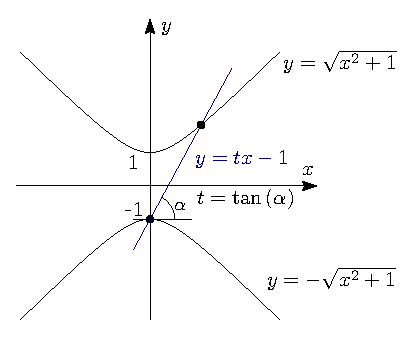
\includegraphics[width=0.4\textwidth]{2_1.eps}
		\caption{Параметризация верхней части гиперболы.}
		\label{2_1}
	\end{figure}
	\uline{Рациональная параметризация}: возьмем точку $-1$ и проведем через нее прямую, пересекающую верхнюю часть гиперболы. Тангенс угла равен $t$, одна точка пересечения это $(0,\SMN 1)$, найдем вторую: 
	$$
		y = tx - 1 \Rightarrow (tx - 1)^2 - x^2 = 1 \Rightarrow t^2 x^2 - 2tx + 1 - x^2 = 1 \Rightarrow x((t^2 - 1)x - 2t) = 0
	$$
	Случай $x = 0$ - отбрасываем, так как это точка $(0,\SMN 1)$, а нас интересует точка пересечения с верхней гиперболой, следовательно:
	$$
		x(t) = \dfrac{2t}{t^2 - 1},\, y(t) = \dfrac{t^2 + 1}{t^2 - 1}
	$$ 
	Таким образом, получили рациональную параметризацию, которая однозначна за исключением одной точки, когда подходим к $\frac{\pi}{2}$ и $t \to \infty$;
	\item Интеграл вида: 
	$$
		\dint R(x, \sqrt{1 - x^2}) \dd x \Rightarrow y = \sqrt{1 - x^2}
	$$ 
	Это верхняя половина окружности, то есть возведя в квадрат получим: $y^2 + x^2 = 1$.
	\begin{rem}
		Одну параметризацию мы знаем - через $\cos{x}$ и $\sin{x}$ (если рассматривать через заметание секторов, то при рассмотрение гиперболы также появляются гиперболические: $\ch{x}, \, \sh{x}$. Как косинусы/синусы задают повороты, так и гиперболические синусы/косинусы будут задавать гиперболические повороты).
	\end{rem}
	\uline{Рациональная параметризация}: возьмем точку $(\SMN 1, 0)$ и проведем через нее прямую, пересекающую верхнюю часть окружности. Снова параметризуем через тангенс:
	$$
		y = (x+1)t \Rightarrow ((x+1)t)^2 + x^2 = 1 \Rightarrow (x+1)^2t^2 = (1-x)(1+x) \Rightarrow 
	$$
	$$
		\Rightarrow (x+1)t^2 = (1-x) \Rightarrow x(t) = \dfrac{1 - t^2}{1 + t^2}
	$$
	Случай $x = -1$ - отбрасываем, так как это $(\SMN1,0)$, а нас интересует $2$-ая точка пересечения, тогда: 
	$$
		x(t) = \dfrac{1 - t^2}{1 + t^2} \Rightarrow y(t) = (x(t) + 1)t = \dfrac{2t}{1 + t^2}
	$$ 
	Следовательно, мы получили запись косинуса и синуса через тангенс половинчатого угла.
	\begin{figure}[H]
		\centering
		\includegraphics[width=0.45\textwidth]{2_2.eps}
		\caption{Параметризация верхней половины окружности.}
		\label{2_2}
	\end{figure}

	Таким образом, получили рациональную параметризацию, которая однозначна за исключением одной точки, когда подходим к $\pi$ и $t \to \infty$;
	\item Интеграл вида: 
	$$
		\dint R(x, \sqrt{x^2 - 1}) \dd x \Rightarrow y = \sqrt{x^2 - 1}
	$$
	Это правая ветвь гиперболы: возведя в квадрат получим $x^2 - y^2 = 1$.
	
	\uline{Рациональная параметризация}: Используем аналогичную предыдущему виду: 
	$$
		y = (x+1)t \Rightarrow x^2 - (x+1)^2t^2 = 1 \Rightarrow (x-1)(x+1) = (x+1)^2t^2 \Rightarrow  x-1 = t^2(x+1) 
	$$
	Таким образом, мы получим следующий результат:
	$$
		 x(t) = \dfrac{1+t^2}{1-t^2}, \, y(t) = \dfrac{2t}{1-t^2}
	$$
\end{enumerate}
\begin{defn}
	Подстановки, приводящие интегралы описанного выше вида к интегралам от рациональных функций называются \uwave{заменами Эйлера}.
\end{defn}

\begin{exrc}\hfill
	\begin{enumerate}[label={(\alph*)}]
		\item Доказать, что $x^3 + y^3 = 1$ не имеет рациональной параметризации;
		\item Обобщить на случай: $x^n + y^n = 1, \, n \geq 3$;
		\item Найти рациональную параметризацию у уравнения: $x^3 + y^3 = xy$;
	\end{enumerate}
\end{exrc}
\begin{proof}\hfill
	\begin{enumerate}[label={(\alph*)}]
		\item Предположим, что такая рационализация существует: 
		$$
			x(t) = \dfrac{p(t)}{r(t)}, \, y(t) = \dfrac{q(t)}{r(t)}
		$$
		где $p(t), q(t), r(t)$ не имеют общего делителя отличного от единицы и следовательно дроби - несократимые. Любую рациональную дробь можно привести к несократимой с точностью до константы. В таком случае, домножив выражение на $r(t)^3$ мы получим следующее: 
		$$
			\bigg(\dfrac{p(t)}{r(t)}\bigg)^3 + \bigg(\dfrac{q(t)}{r(t)}\bigg)^3 = 1 \Rightarrow p(t)^3 + q(t)^3 = r(t)^3
		$$ 
		тогда $p(t), q(t), r(t)$ будут взаимно простыми, иначе был бы общий делитель отличный от единицы. Продифференцируем это уравнение, получим:
		$$
			p^2 p^\prime + q^2 q^\prime - r^2r^\prime = 0 
		$$
		Можем предположить, что $\deg{p} \geq \deg{q} \wedge \deg{p} \geq \deg{r}$. Домножим выражение на $r$ и получим:
		$$
			p^2p^\prime r + q^2 q^\prime r - r^3 r^\prime = p^2(rp^\prime - pr^\prime) + q^2 (qr^\prime - rq^\prime) = 0 \Leftrightarrow p^2(rp^\prime - pr^\prime) = q^2 (rq^\prime - qr^\prime ) 
		$$
		Если хотя бы одна из частей равенства равна $0$, то $\tfrac{p(t)}{r(t)}$ и $\tfrac{q(t)}{r(t)}$ будут равны константам, поскольку:
		$$
			\left( \dfrac{p}{r} \right)^\prime = \dfrac{rp^\prime - pr^\prime}{r^2} = 0 \Leftrightarrow rp^\prime - pr^\prime = 0, \, \left( \dfrac{q}{r} \right)^\prime = \dfrac{rq^\prime - qr^\prime}{r^2} = 0 \Leftrightarrow rq^\prime - q r^\prime = 0
		$$
		и тогда $q(t) = kr(t)$ и $p(t) = mr(t)$, что будет противоречить несократимости дроби. 
		
		Поскольку $p(t)$ и $q(t)$ взаимно просты и при делении выражения $q^2 (rq^\prime - qr^\prime )$ на $p^2$ мы получаем многочлен, то $(rq^\prime - q r^\prime)$ делится на $p^2$, то есть:
		$$
			2\deg{p} \leq \max\{\deg{r} + \deg{q} - 1, \deg{r} - 1 + \deg{q}\} = \deg{r} + \deg{q} - 1
		$$
		что невозможно, поскольку:
		$$
			2\deg{p} \geq \deg{q} + \deg{r}
		$$ 
		тогда: $\deg{p} < \deg{r} \vee \deg{p} < \deg{q}$, аналогично получим, что: 
		$$
			\deg{r} < \deg{q} \vee \deg{r} < \deg{p}, \, \deg{q} < \deg{r} \vee \deg{q} < \deg{p}
		$$ 
		что невозможно $\Rightarrow$ приходим к противоречию с тем, что такая рациональная параметризация существует. Случаи, когда одно из слагаемых равно константе входят в этот случай. Если отношение хотя бы двух слагаемых равно константе, тогда это не является параметризацией, поскольку получаем одну точку;
		\item В общем случае, рассуждения аналогичные, выражение полученное при дифференцировании будет следующим:
		$$
			p^{n-1}p^\prime  + q^{n-1}q^\prime - r^{n-1}r\prime = 0 \Leftrightarrow p^{n-1}(rp^\prime - pr^\prime) = q^{n-1}(qr^\prime - rq^\prime)
		$$
		И при аналогичных рассуждения про степень многочленов мы придем к противоречию;
		
		\item Предположим, что $y = xt$, подставив в исходное выражение мы получим следующее:
		$$
			x^3 + t^3x^3 = tx^2 \Leftrightarrow x^3(1+t^3) = x^2 t \Leftrightarrow x(t) = \dfrac{t}{1+t^3}, \, y(t) = \dfrac{t^2}{1+t^3}
		$$
		Пусть $x(t) = \dfrac{t}{1 + t^3}, \, y(t) = \dfrac{t^2}{1+t^3}$, тогда подставляя это в уравнение получим:
		$$
			x(t)^3 + y(t)^3 = \dfrac{t^3}{(1+t^3)^3} + \dfrac{t^6}{(1+t^3)^3} = \dfrac{t^3(1+t^3)}{(1+t^3)^3} = \dfrac{t^3}{(1+t^3)^2} = x(t){\cdot}{y(t)}
		$$
	\end{enumerate}
\end{proof}

\section*{Интегрирование тригонометрических функций}
$$
	\dint R(\cos{x}, \sin{x}) \dd x
$$ 
В интегралах подобного типа есть \uline{универсальная замена}: 
$$t = \tg{\frac{x}{2}} \Rightarrow \cos{x} = \dfrac{1-t^2}{1+t^2},\, \sin{x} = \dfrac{2t}{1+t^2} \Rightarrow x = 2\arctan{t} \Rightarrow \dx = \dfrac{2}{1+t^2} \dd t$$
Таким образом, все что получится после подстановки будет рациональной функцией от $t$.
\begin{rem}
	Всегда нужно смотреть, а нужна ли вообще такая замена? Как в случаях: 
	$$
		\dint \sin{x} \dx \vee \dint R(\cos^2{x}, \sin{x})\cos{x} \dx
	$$
	где нужна замена всего на $\sin{x}$.
\end{rem}

\subsection*{Примеры интегралов, которые не выражаются в элементарных функциях}
Типичные примеры интегралов, которые не выражаются в элементарных функциях: 
$$\dint e^{x^2}\dx, \, \dint \dfrac{\sin{x}}{x}\dx, \, \dint \dfrac{e^x}{x}\dx$$
Как выяснить берется интеграл или нет? Ответ на этот вопрос базируется на теореме Лиувилля. В данном курсе её рассматривать не будем, но упомянем про её суть.

\textbf{\uline{Элементарные функции}}: $x^n, \, e^x, \, \ln{x}, \, \cos{x}, \, \sin{x}, \, \arcsin{x}, \, \arccos{x}, \, \arctg{x}, \, \arcctg{x}, \, \sqrt[m]{x}$. При интегрировании ответ получается составлен из элементарных функций, алгебраических операций: $+,\, -,\, \cdot,\, / $ и композиции этих функций.

Было сделано несколько наблюдений:
\begin{enumerate}[label={(\arabic*)}]
	\item Полезно перейти к комплексным числам и оставить очень короткий список функций: рациональные функции, $e^z$ и $\ln{z}$. Например: 
	$$
		\cos{x} = \dfrac{e^{ix} + e^{-ix}}{2}
	$$ 
	Если захотим найти обратную функцию, то: 
	$$
		\dfrac{e^{ix} + e^{-ix}}{2} = t \Rightarrow (e^{ix})^2 - 2 e^{ix}t + 1 = 0 
	$$ 
	Решаем квадратное уравнение. Корни можно искать, как $x^p = e^{p\ln{x}}$;
	\item Операцию композиции можно выразить алгебраически: поскольку список функций стал меньше, то необходимо научиться брать композицию какой-нибудь полученной на предыдущем шаге функции с экспонентой и какой-нибудь полученной на предыдущем шаге функции с  логарифмом;
\end{enumerate}

Как брать композиции? Сложную операцию подстановки одной функции в другую можно рассматривать как решение уравнения в элементарных функциях. 

Были рациональные функции $\Rightarrow$ расширяем на решения алгебраических уравнений - алгебраическое расширение: были решения в $\MQ$ добавили квадратный корень $\Rightarrow a\sqrt{2} + b$ - расширение; или было $\MR$, расширяем на решения $x^2 + 1 = 0 \Rightarrow ai + b$ - расширение. То есть, с помощью дифференциальных уравнений умеем добавлять экспоненту и логарифм. Например: 
$$
	f = e^g \Leftrightarrow f^\prime = f{\cdot}g^\prime
$$
Таким образом, экспоненту и логарифм функции можно определить как решение дифференциального уравнения;

\begin{defn}
	Будем говорить, что функция \uwave{элементарна}, если мы можем за конечное число шагов, используя решения алгебраических уравнений и операции композиции с экспонентами и логарифмами, получить эту функцию из рациональной функции.
\end{defn}
\textbf{Пример}: $e^{P(x)}$ - это элементарная функция, где $P(x)$ - многочлен.

Сама теорема говорит о том, что интеграл возьмется, только если подинтегральная функция имеет специальный вид. И проверка, что какие-то интегралы не берутся в элементарных функциях происходит с помощью доказательства того, что подинтегральное выражение такого вида иметь не может.
\end{document}